\section{Experiments and Results}
\label{sec:experiments}

\subsection{Experimental Setup}
We evaluate the greedy policy and two beam search lookahead policies using the Willow Garage PR2 robot in a simulation environment on the task of tying an overhand knot.

\subsubsection{Demonstrations}
We use the set of demonstrations collected by \citet{Schulmanetal_ISRR2013} for their rope-tying experiments.
These demonstrations were collected in the real world and consist of 148 pairs of point clouds and gripper trajectories.
The point clouds were collected using an RGBD camera and then filtered based on color to remove the green background of the table, and leave only the point cloud representation of the rope.
The gripper trajectories were recorded kinesthetically, from human-guided demonstrations that move the robot's grippers to tie a knot.
The dataset contains demonstrations for a three steps method of tying an overhand knot and recovery demonstrations that
enable recovery from common failures.

\subsubsection{Simulation Environment for Knot Tying} 
The training, validation, and evaluation of our policy are run in simulation.
The simulation environment uses Bullet Physics~\cite{Bullet_Physics} as the physics engine.
The rope is simulated with a linked chain of capsules with bending and torsional constraints.

\subsubsection{Benchmark}
For the labeled examples \labelset{} used to train our \mmql{} model, we experiment with both human-labeled examples 
and automatically generated leave-one-out labeled examples.
In both cases, an example is a pairing of a point cloud and an optimal action.
For the human-labeled examples, we use traces of complete task executions, from a randomly drawn initial 
rope configuration to a successfully tied knot.
% TODO: Add description of how we choose the best action
Each example contains a reference to its predecessor, so we can represent the associated Bellman equations.

Initial rope states are randomly perturbed configurations of uniformly drawn samples from the initial rope states in the demonstration library.
The process of perturbing a rope state consists of selecting five uniformly-spaced points along the rope and dragging each in a random direction for a random radius between 0 and 15 cm.
All initial rope configurations in our experiments are drawn from this distribution.

Our labeling interface shows the user simulations of applying demonstrations in decreasing order a registration cost, which is a rough measure of the quality of an action.
When human labeler see an action that she deems optimal (or close enough to optimal) she indicates that, the simulated robot commits to that action and the process 
proceeds until a knot is tied.
The leave-one-out labeled examples are generated as outlined in Section~\ref{subsec:lool}. 

In addition, the benchmark contains an evaluation set of 500 randomly drawn initial configurations. 
We define success to be tying an overhand knot in a sequence of 5 or fewer actions.

\subsection{Experiments}
We evaluate the success rate using the following policies when using the expert-labeled and leave-one-out labeled examples: greedy, one-step lookahead with width 10, and two-step lookahead with width 5.
\subsubsection{Expert-labeled Examples}
For this evaluation, 1000 expert-labeled examples are used.
For each of these policies, the optimization hyperparameters $C$, $D$ and $F$ are first tuned via holdout 
validation, using a holdout set of 100 randomly drawn initial rope states (distinct from the evaluation set). 
For this case, the best-performing hyperparameters we found are $C=2$, $D=1$ and $F=1$.
We applied \mmql{} with these hyper-parameter settings and ran each of the three policies 
on the evaluation set.
As a baseline comparison, we also evaluate using the nearest neighbor policy presented in \citet{Schulmanetal_ISRR2013}.
Their policy chooses the action associated with the state that has the smallest registration cost with respect to the current state.
The success rates obtained under these policies are summarized in Table~\ref{table:performance}. Note that our best results surpass the baseline by 26.4\%.
Almost two-thirds of this improvement results from the greedy approach of choosing the action that
maximizes the Q-value, given the current state. The remaining improvement is gained through lookahead; the
performance of depth 1, width 10 lookahead and depth 2, width 5 lookahead are approximately the same (Table~\ref{table:performance}).

\begin{table}
  \centering
  \begin{tabular}{lc}
    \toprule
      Policy & Success Rate\\
    \midrule
      Nearest neighbor \cite{Schulmanetal_ISRR2013} & 68.8\% \\
    \midrule
      Greedy & 85.6\% \\
      Lookahead (depth 1, width 10) & 93.6\% \\
      Lookahead (depth 2, width 5) & 95.2\% \\
    \bottomrule
  \end{tabular}
  \caption{Success rate of tying a knot using the expert-labeled examples. The neareast-neighbor method selects
           the demonstration that minimizes a bi-directional registration cost associated with the trajectory transfer.
           Other policies maximize the approximate Q-function we learn through \mmql{}. Greedy maximizes this value in the current
           state. The lookahead policies act to maximize a back up value computed by beam search with the specified parameters. The greedy
           succeeds in an additional 17\% of examples when compared with the baseline. Lookahead policies achieve very high performance rates
           and approach the best possible with our demonstration library.}
  \label{table:performance}
\end{table}

The approximate values of the states for the 500 evaluated runs in the validation set are plotted in Figure~\ref{fig:values} as a function of time steps 1 through 5.
Observe that Q values are generally increasing; we expect this since the Bellman constraints in our formulation pushes states closer to the goal to have higher values.
Also, recall that the state value of the tied knot is close to zero, which is visible in the figure (Equation~\ref{eq:bellman_goal_constr}).
For most of the runs, the policy is able to reach the goal state in 3 steps, which is optimal since the expert took a minimum of three actions to tie a knot.
Examination of the baseline graph shows that, even in the cases where it successfully ties a knot, it often requires 4 steps to do so, demonstrating that our learned
policy is able to more quickly tie a knot in additional to being more robust.

\begin{figure}
  \centering
  \begin{subfigure}[b]{0.48\linewidth}
    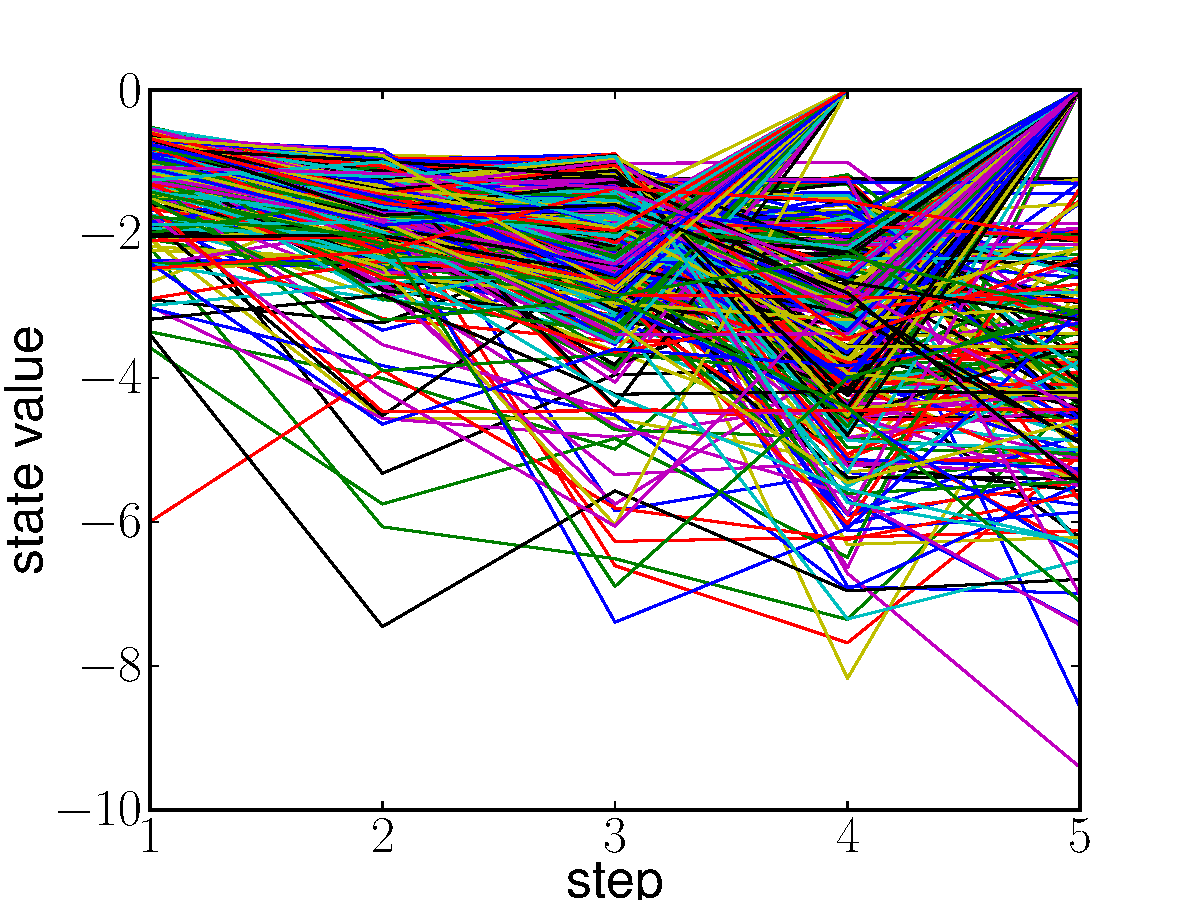
\includegraphics[width=\textwidth]{figures/state_value_baseline.pdf}
    \caption{baseline}
    \label{fig:value_baseline}
  \end{subfigure}
  \begin{subfigure}[b]{0.48\linewidth}
    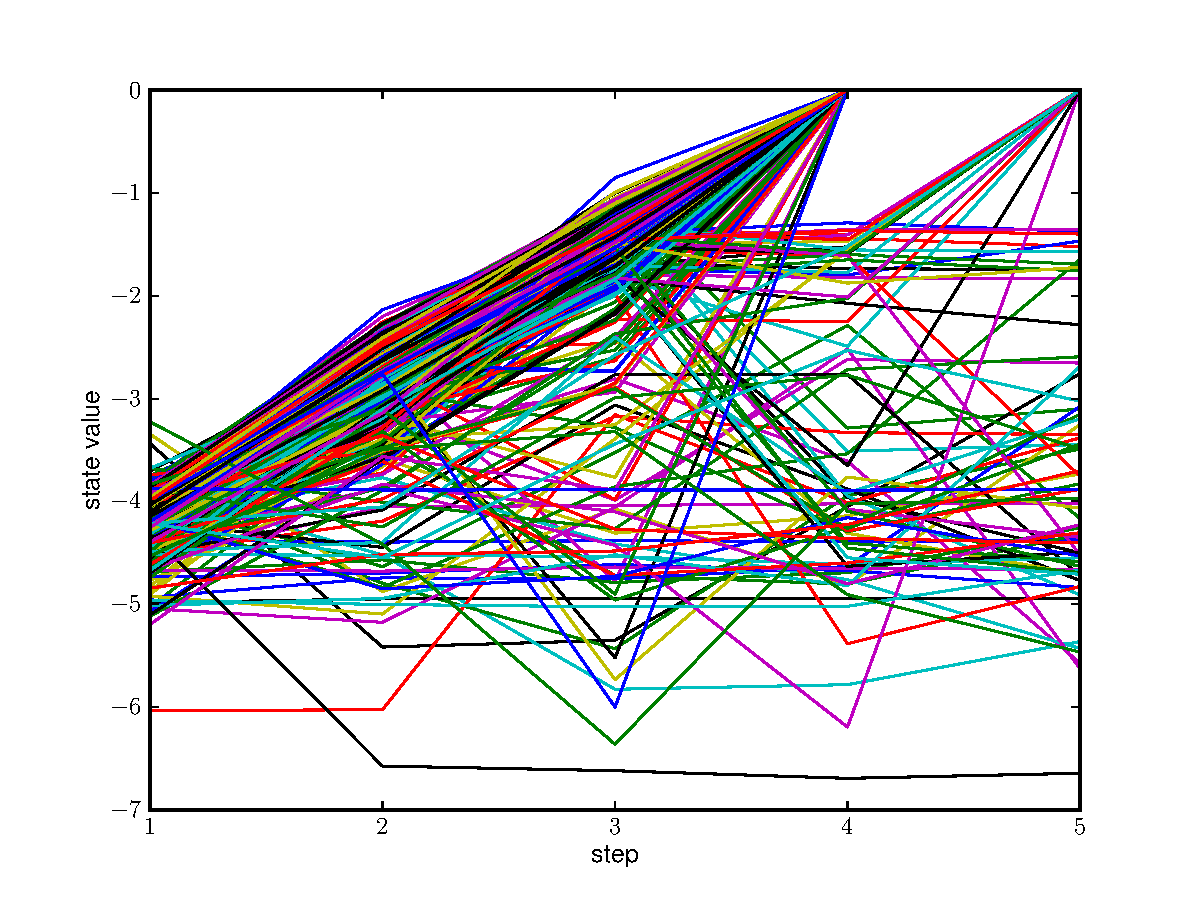
\includegraphics[width=\textwidth]{figures/state_value_greedy.pdf}
    \caption{greedy}
    \label{fig:value_greedy}
  \end{subfigure}
  \begin{subfigure}[b]{0.48\linewidth}
    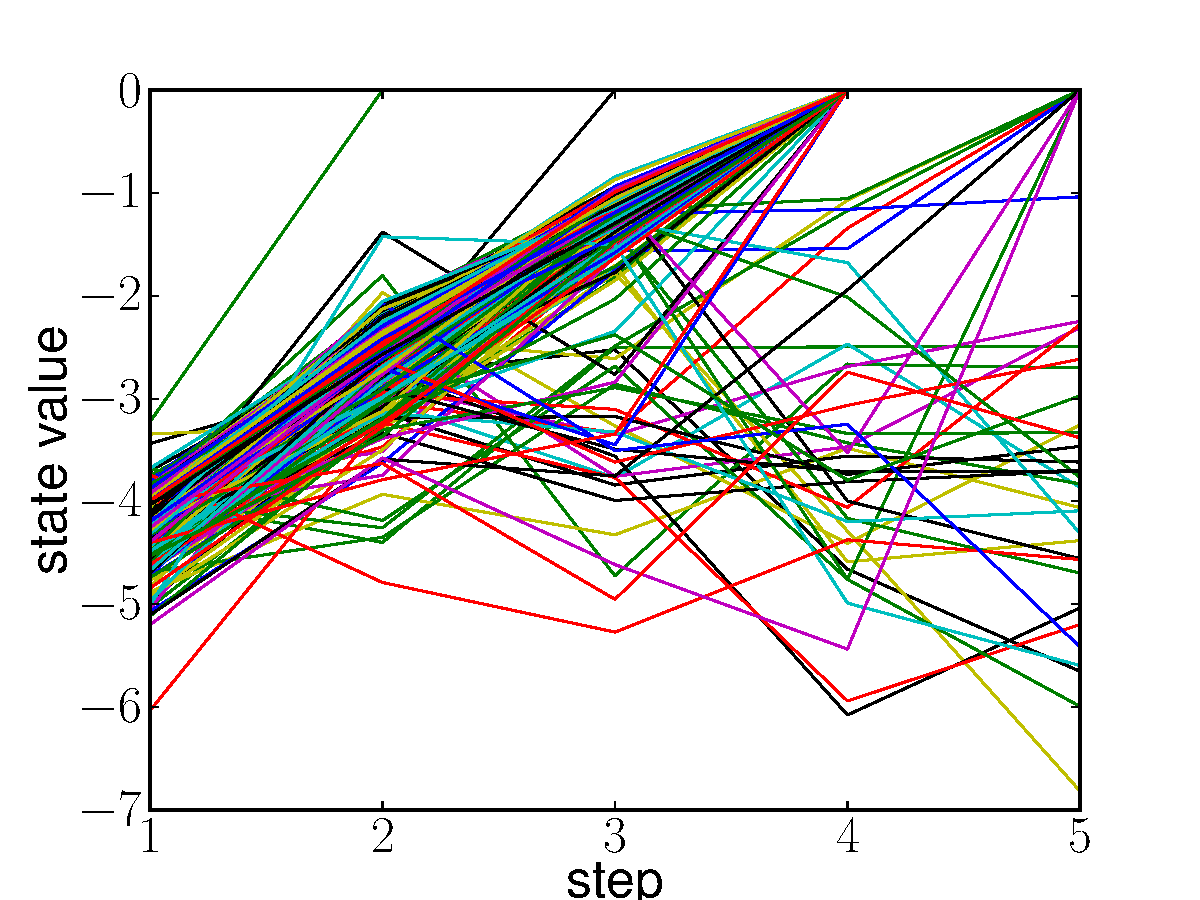
\includegraphics[width=\textwidth]{figures/state_value_lookahead1-10.pdf}
    \caption{lookahead (depth 1, width 10)}
    \label{fig:value_lookahead_1}
  \end{subfigure}
  \begin{subfigure}[b]{0.48\linewidth}
    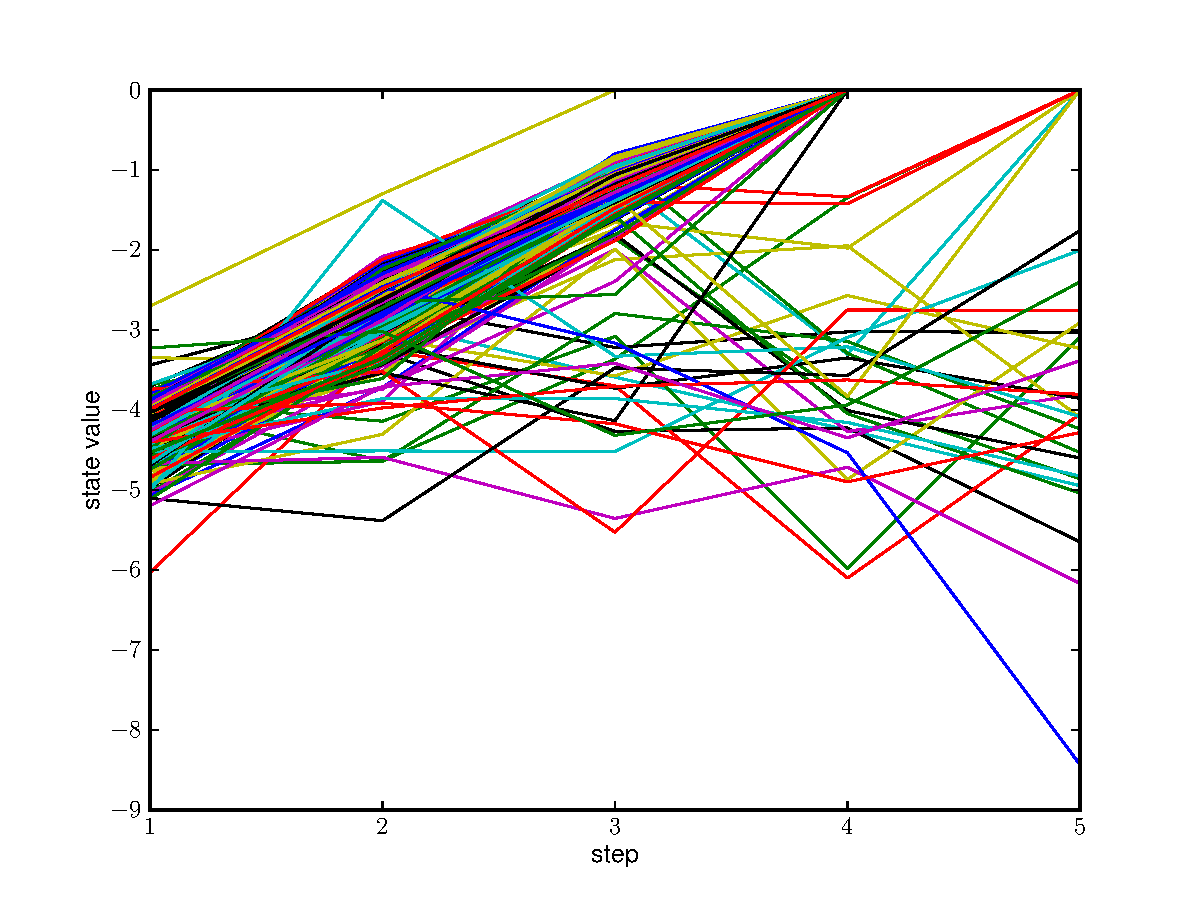
\includegraphics[width=\textwidth]{figures/state_value_lookahead2-5.pdf}
    \caption{lookahead (depth 2, width 5)}
    \label{fig:value_lookahead_2}
  \end{subfigure}
  \caption{Plots of Q values over executions on the evaluation set. The x-axis indicates which step in the execution
           the evaluation comes from. A value of 0 corresponds to successfully tying a knot. For comparison, we show the 
           negative registration cost of the nearest-neighbor baseline. The structure in our learned function can be seen
           in the strong upward trend in Q-values as execution progresses. The lack of structure in the nearest-neighbor
           motivates the need to Q-function learning: minimizing registration cost in a forward search will \emph{harm} performance.}
  \label{fig:values}
\end{figure}

We also examine the relation between the number of expert-labeled examples and
the success rate for each of the four policies, including the nearest-neighbor
baseline policy.  These success rates are shown in
Table~\ref{table:number_examples}.  As expected, the success rate increases as
we use more labeled examples. However, the resulting policies remain
surprisingly resilient. Even with only 50 training examples, the greedy policy is able to beat the baseline by over 12\%.

\begin{table}
  \centering
  \begin{tabular}{lc}
    \toprule
      \# of Training Examples & Success Rate\\
    \midrule
      Nearest neighbor \cite{Schulmanetal_ISRR2013} & 68.8\% \\
    \midrule
      50 & 81.2\% \\
      100 & 85.2\% \\
      500 & 84.6\% \\
      1000 & 85.6\%\\
    \bottomrule
  \end{tabular}
  \caption{We vary the number of examples used to generate constraints for the
    \mmql{} optimization problem and examine how task performance is affected
    over 500 test trials using the resulting greedy policy. It turns out that
    the number of examples has a relatively small influence on the performance
    of the resulting policy.}
  \label{table:number_examples}
\end{table}

\subsubsection{Leave-One-Out Labeled Examples}

After holdout validation and evaluation, done in the same manner as our main
experiment, we find that learning a greedy policy with a leave-one-out labeled
example set achieves a performance of 78.0\%, a drop of 7.6\% from our
supervised result. However, this result still surpasses the baseline by
9.2\%. This indicates that, if expert demonstrations are in short supply, one
can still improve significantly over a na\"{\i}ve nearest-neighbor policy by
training with an example set generated through leave-one-out labeling.

We do not present results for lookahead policies. Because the
automatically-generated example set does not have temporal information, the
optimization problem used to derive a greedy policy does not contain Bellman
constraints. The absence of these constraints makes the resulting weight vector
ill-suited for performing lookahead.
